%----------------------------------------------------------------------------------------
%    PACKAGES AND THEMES
%----------------------------------------------------------------------------------------

\documentclass[aspectratio=169,xcolor=dvipsnames]{beamer}
\usetheme{SimpleDarkBlue}

\usepackage{hyperref}
\usepackage{graphicx} % Allows including images
\usepackage{booktabs} % Allows the use of \toprule, \midrule and \bottomrule in tables

%----------------------------------------------------------------------------------------
%    TITLE PAGE
%----------------------------------------------------------------------------------------

\title{Evaluating Investment Strategies: Beyond Buy and Hold}
\subtitle{A Quantitative Analysis of S\&P 500 and Bond Yields}

\author{Farhan Sadeek. Jalen Francis, Jayson Clark \texorpdfstring{\\}{,} Adhitya Bhati, Andrew McKenzie}

\institute
{
    Department of Mathematics \\
    The Ohio State University % Your institution for the title page
}
\date{\today} % Date, can be changed to a custom date

%----------------------------------------------------------------------------------------
%    PRESENTATION SLIDES
%----------------------------------------------------------------------------------------

\begin{document}

\begin{frame}
	% Print the title page as the first slide
	\titlepage
\end{frame}

\section{Market Classification}
\begin{frame}{Market Classification}
	\begin{itemize}
		\item \textbf{Objective}: Classify market states (Bear, Bull, Static) using S\&P 500 data.
		\item \textbf{Methodology}:
		      \begin{itemize}
			      \item Calculate rolling peak and trough.
			      \item Bear: Drawdown from peak > 20\%.
			      \item Bull: Increase from trough > 20\%.
			      \item Static: Neither Bear nor Bull.
		      \end{itemize}
		\item \textbf{Implementation}:
		      \begin{itemize}
			      \item Python with Pandas, NumPy, Matplotlib.
			      \item Logging and visualization.
		      \end{itemize}
		\item \textbf{Results}:
		      \begin{itemize}
			      \item Market state distribution.
			      \item Plot of S\&P 500 with market states.
		      \end{itemize}
	\end{itemize}\end{frame}\begin{frame}{Market Classification}
	\begin{figure}
		\centering
		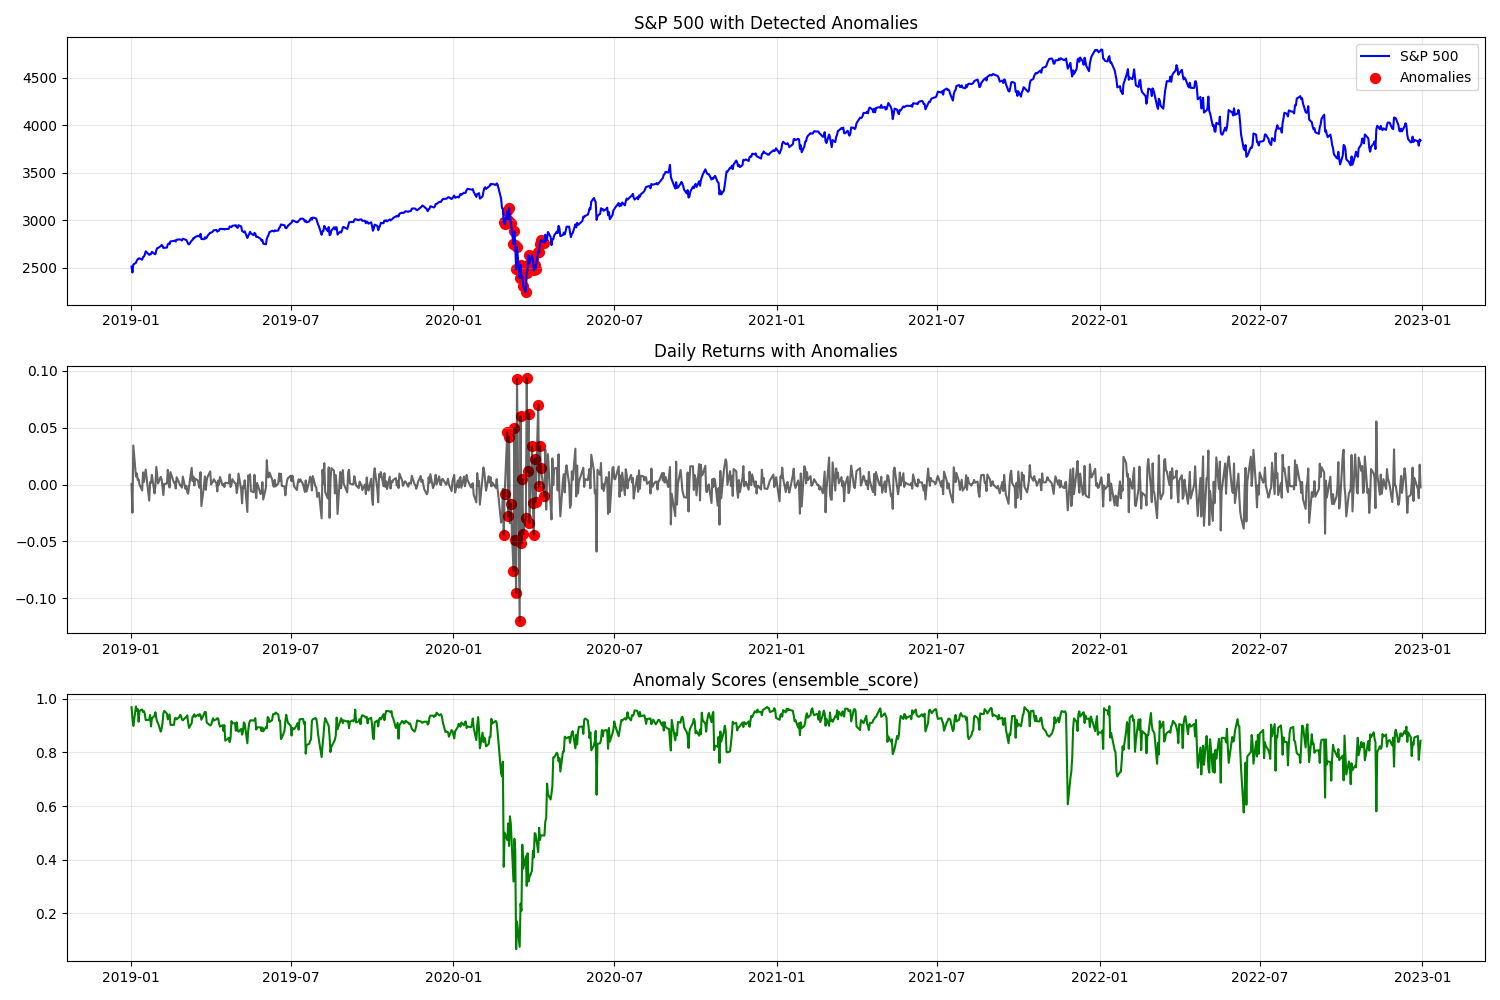
\includegraphics[width=0.8\textwidth]{anomalies_visualization.png}
		\caption{S\&P 500 with Market State Classification}
	\end{figure}
\end{frame}
%------------------------------------------------
\section{Why Neural Network?}
\begin{frame}{Why Neural Networks for Investment Strategy?}
	\begin{itemize}
		\item Neural networks can identify complex patterns in financial data that traditional models are very likely miss
		\item Our approach avoids hard-coded investment rules, allowing the model to learn optimal strategies directly from historical market data
		\item This data-driven methodology adapts to changing market conditions more effectively than static strategies
		\item The model incorporates multiple factors simultaneously, capturing nuanced relationships between S\&P 500 movements and bond yields
	\end{itemize}
\end{frame}
%------------------------------------------------
\section{Anomaly Detection}
\begin{frame}{Anomaly Detection}
	While creating our model, we realized that there might be certain market conditions that might affect the performance of our investment strategies. For example, in our case, there was the COVID-19 pandemic, which caused the market to perform abruptly. In order to account for that, we developed a neural network that will detect the anomaly and avoid those pitfalls. You can find our analysis on that in \texttt{market\_anomaly.py}
\end{frame}
\begin{frame}{Anomaly Detection}
	\begin{figure}
		\centering
		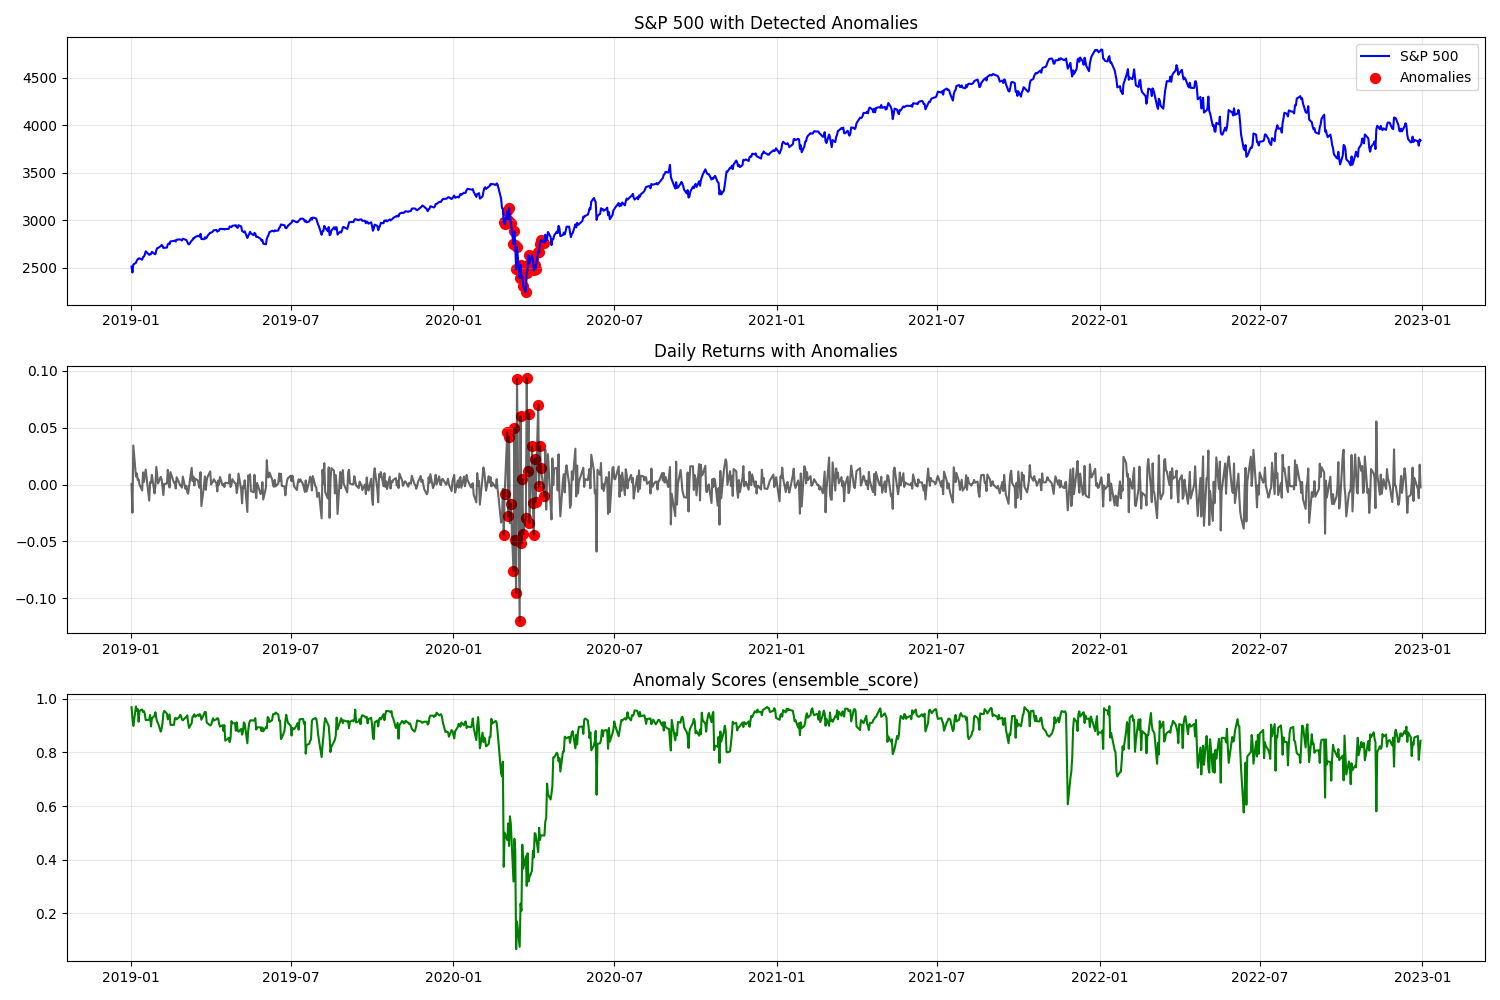
\includegraphics[width=0.8\textwidth]{anomalies_visualization.png}
		\caption{S\&P 500 with Market State Classification}
	\end{figure}
\end{frame}
\begin{frame}{Overview}
	% Throughout your presentation, if you choose to use \section{} and \subsection{} commands, these will automatically be printed on this slide as an overview of your presentation
	\tableofcontents
\end{frame}


\section{Problem Statement}
\begin{frame}{Problem Statement}
	Although buying and holding is considered the best strategy in investing. We would have to prove or disprove that hypothesis based on the dataset given to us about the price of S\&P 500 and bond yield rate.
\end{frame}
\section{Our Solution}
\begin{frame}{Our Solution}
	We will disprove this hypothesis by coming up with our own investment strategy that minimizes risk while maximizing returns. By employing a mixed-methods approach that combines statistical analysis with machine learning techniques, we aim to identify potential patterns and trends within the financial data that can inform our investment strategy. Specifically, we will analyze historical price movements of the S\&P 500 alongside various economic indicators, including bond yield rates, to uncover correlations that may suggest more optimal entry and exit.
\end{frame}
%------------------------------------------------
\section{Our approach}
%------------------------------------------------

\begin{frame}{Bullet Points}

	\begin{itemize}
		\item Lorem ipsum dolor sit amet, consectetur adipiscing elit
		\item Aliquam blandit faucibus nisi, sit amet dapibus enim tempus eu
		\item Nulla commodo, erat quis gravida posuere, elit lacus lobortis est, quis porttitor odio mauris at libero
		\item Nam cursus est eget velit posuere pellentesque
		\item Vestibulum faucibus velit a augue condimentum quis convallis nulla gravida
	\end{itemize}
\end{frame}

%------------------------------------------------


%------------------------------------------------
\begin{frame}{Blocks of Highlighted Text}
	In this slide, some important text will be \alert{highlighted} because it's important. Please, don't abuse it.

	\begin{block}{Block}
		Sample text
	\end{block}

	\begin{alertblock}{Alertblock}
		Sample text in red box
	\end{alertblock}

	\begin{examples}
		Sample text in green box. The title of the block is ``Examples".
	\end{examples}
\end{frame}

%------------------------------------------------

\begin{frame}{Multiple Columns}
	\begin{columns}[c] % The "c" option specifies centered vertical alignment while the "t" option is used for top vertical alignment

		\column{.45\textwidth} % Left column and width
		\textbf{Heading}
		\begin{enumerate}
			\item Statement
			\item Explanation
			\item Example
		\end{enumerate}

		\column{.45\textwidth} % Right column and width
		Lorem ipsum dolor sit amet, consectetur adipiscing elit. Integer lectus nisl, ultricies in feugiat rutrum, porttitor sit amet augue. Aliquam ut tortor mauris. Sed volutpat ante purus, quis accumsan dolor.

	\end{columns}
\end{frame}

%------------------------------------------------
\section{Second Section}
%------------------------------------------------

\begin{frame}{Table}
	\begin{table}
		\begin{tabular}{l l l}
			\toprule
			\textbf{Treatments} & \textbf{Response 1} & \textbf{Response 2} \\
			\midrule
			Treatment 1         & 0.0003262           & 0.562               \\
			Treatment 2         & 0.0015681           & 0.910               \\
			Treatment 3         & 0.0009271           & 0.296               \\
			\bottomrule
		\end{tabular}
		\caption{Table caption}
	\end{table}
\end{frame}

%------------------------------------------------

\begin{frame}{Theorem}
	\begin{theorem}[Mass--energy equivalence]
		$E = mc^2$
	\end{theorem}
\end{frame}

%------------------------------------------------

\begin{frame}{Figure}
	Uncomment the code on this slide to include your own image from the same directory as the template .TeX file.
	%\begin{figure}
	%\includegraphics[width=0.8\linewidth]{test}
	%\end{figure}
\end{frame}

%------------------------------------------------


%------------------------------------------------

\begin{frame}
	\Huge{\centerline{\textbf{The End}}}
\end{frame}

%----------------------------------------------------------------------------------------

\end{document}